\documentclass[10pt]{beamer}

\usetheme[progressbar=frametitle]{metropolis}
\usepackage{appendixnumberbeamer}

\usepackage{booktabs}
\usepackage[scale=2]{ccicons}
\usepackage{fontawesome}
\usepackage{pgfplots}
\usepgfplotslibrary{dateplot}
\usepackage{mathtools}
\usepackage{xspace}
\newcommand{\themename}{\textbf{\textsc{metropolis}}\xspace}
%\usepackage{caption}
%\usepackage{hyperref}
%\usepackage[citestyle=authoryear,natbib=true,backend=bibtex]{biblatex}
%\usepackage{biblatex}
%\bibliography{rl}
%\usepackage{natbib}

\title{A Brief Survey of Reinforcement Learning}
\subtitle{A modern beamer theme}
\date{\today}
% \date{11 Dec 2018}
\author{Giancarlo Frison}
%\institute{ \faTwitter gfrison}
% \titlegraphic{\hfill\includegraphics[height=1.5cm]{logo.pdf}}
\begin{document}

\setbeamertemplate{frame footer}{\faTwitter gfrison 2018}

\maketitle

\begin{frame}{Table of contents}
  \setbeamertemplate{section in toc}[sections numbered]
  \tableofcontents[hideallsubsections]
\end{frame}

\section{Introduction}
\begin{frame}[fragile]{What is Reinforcement Learning}
	\begin{figure}[t!]	
	\centering
	\includegraphics[scale=0.3]{img/donkey.png}
	\cite{donkey}
	\end{figure}
	\textsc{Reinforcement learning} is an area of machine learning concerned with how software agents ought to take actions in an environment so as to maximize some notion of cumulative reward.
\end{frame}

\begin{frame}[fragile]{Challenges in RL}
	RL  vision  is about creating  systems that  are  capable  of  learning  how  to  adapt  in  the  real  world, solely based on trial-and-error.
	
	Challenges:
	\begin{itemize}
		\item The  optimal  policy  must  be  inferred  by  interacting with the environment. The only learning signal
the agent receives is the reward.
		\item Agents  must  deal  with  long-range  time  dependencies:
Often the consequences of an action only materialise after
many transitions of the environment \cite{Montague1999}.
	\end{itemize}
\end{frame}

\begin{frame}[fragile]{What it is Not}
Although RL can induce to an optimization, there are major differences within:
  \begin{itemize}[<+- | alert@+>]
    \item {Supervised learning}
	\item Mathematical optimization
	\item Genetic programming
  \end{itemize}
\end{frame}

\section{Genetic Programming}
\begin{frame}{Genetic Programming}
	\textsc{GP} is a technique whereby computer programs are encoded as a set of genes that are then modified using an evolutionary algorithm.
	\begin{itemize}
		\item A number of chromosomes are randomly created.
		\item Each chromosome is evaluated through a fitness function.
		\item Best ones are selected, the others are disposed.
		\item Chromosomes could be breded among the selected for a new generation.
		\item Offsprings are randomly mutated.
		\item Repeat until the score threshold is reached \cite{gf-gp}.
	\end{itemize}
\end{frame}

\begin{frame}{Crossover}
	\begin{figure}
		\includegraphics[scale=0.15]{img/ast-crossover.png}
		\caption{The “breeding” is called crossover. The chromosome (in this case an \textsc{AST}), is merged between two individuals for searching a better function.}
	\end{figure}	
\end{frame}

\begin{frame}{Strenghts on many local minima}
\textsc{GP} may overtake gradient-based algorithms when the solution space has many local minima
	\begin{figure}
		\includegraphics[scale=0.16]{img/Rastrigin_function.png}
		\caption{Rastrigin function}
	\end{figure}
\end{frame}

\begin{frame}{Strenghts on no-differentiable functions}
$f(x)$ is \textsc{differentiable} when it has always a finite derivative along the domain. 
	\begin{figure}
		\begin{tikzpicture}[scale=0.5]
			\begin{axis}[
			    xmin=-2, xmax=2,
			    ymin=-1, ymax=2,
			    axis lines=center,
			    axis on top=true,
			    domain=-1:1,
			    ]
			
			    \addplot [mark=none,draw=red,ultra thick] {abs(x)};
			\end{axis}
		\end{tikzpicture}
	    \caption{$f(x) = |x|$ has no derivative at $x = 0$.}
	\end{figure}
\textsc{GP} is not sensitive on \emph{latent} no-differentiable functions.	
\end{frame}

\section{Multi-armed Bandit}
\begin{frame}{Multi-armed Bandit}
	\begin{figure}[t!]	
	\centering
	\includegraphics[scale=0.2]{img/Las_Vegas_slot_machines.jpg}
	\end{figure}
	The multi-armed bandit problem has been the subject of decades of intense study in statistics, operations research, electrical engineering, computer science, and economics \cite{bandit}
\end{frame}

\begin{frame}
	\frametitle{\begin{math} Q \end{math} Value's Action}
	\begin{figure}[t!]
		\centering
		\includegraphics[scale=0.25]{img/bandit-reward-dist.png}
	\end{figure}
	An example bandit problem \cite{Montague1999}. Obtained measures after repeated pullings with 10 arms.
\end{frame}

\begin{frame}
	\frametitle{\begin{math} Q \end{math} Value's Action}
	\begin{math} \mathbf{Q_n} \end{math} is the estimated value of its action after $ n $ selections.	
	$$ Q_{n+1} = \frac{R_1 +R_2 + ... +R_{n}}{n} $$
	A more scalable formula, updates the average with incremental and small constant:
	$$ Q_{n+1} = Q_n + \frac{1}{n}(R_n-Q_n)$$
	General expression of the badint algorithm at the fundation of RL. \begin{math}Target\end{math} could be considered the reward $ R $ by now.
	$$ \mathbf{NewEstimate = OldEstimate + StepSize(Target-OldEstimate)}$$
\end{frame}

\begin{frame}
\frametitle{Gambler's Dilemma}
When pulled, an arm produces a random payout drawn independently of the past. Because the distribution of payouts corresponding to each arm is not listed, the player can learn it only by experimenting.
	\begin{columns}
		\begin{column}{0.5\textwidth}
			\begin{alertblock}{Exploitation}
		Earn more money by exploiting arms that yielded high payouts in the past.
			\end{alertblock}
		\end{column}
		\begin{column}{0.5\textwidth}  %%<--- here
			\begin{alertblock}{Exploration}
		Exploring alternative arms may return higher payouts in the future.
			\end{alertblock}
		\end{column}
	\end{columns}
\end{frame}

\section{Markov Decision Process}
\begin{frame}
	\frametitle{Definition of MDP}
	\begin{figure}
		\includegraphics[scale=0.15]{img/2015_DARPA_Robotics_Challenge_150606-N-PO203-090.jpg}	
		\caption{2015 DARPA Robotics Challange \cite{mdp-robot}}
	\end{figure}
	Despite as in bandits, MDP formalizes the decision making (Policy $\pi$) in sequential steps, aggregated in Episodes. 
\end{frame}

\begin{frame}
	\frametitle{Actions and States}
	\begin{figure}
	\includegraphics[scale=0.2]{img/mdp-states.png}
	\caption{Model representation of MDP \cite{mdp-process}}
	\end{figure}
	MDP strives to find the best $\pi$ to all possible states. 
	In Markov processes, the selected action depends \textbf{only} on current state.
\end{frame}

\begin{frame}
	\frametitle{How to evaluate an Agent?}
	Given that:
	\begin{itemize}
		\item Policy $\pmb{\pi}$ defines a particular way of acting.
		\item $\mathbf{v_π(s)}$ is the expected return from $\mathbf{s}$ following $\pmb{\pi}$ \emph{thereafter}.
		\item $\mathbf{q_π(s, a)}$ is the $\mathbf{v_π(s)}$ taking action $\mathbf{a}$
		\item For maximizing future rewards, only the $\mathbf{max}$ $Q_\pi$ is considered. 
		\item $\pmb{\gamma}$ is the rewards' discount factor. 
	\end{itemize}
	
	A recursive algorithm could be indentified, known as the \textsc{Bellman equation}. Iteratevely computes the value $\mathbf{Q}$ from the terminal state:
	$$ \mathbf{Q_t(s, a) = R_{t + 1} + \gamma max[v(S_{t+1})]} $$

	
		
\end{frame}

\begin{frame}
	\frametitle{Grid World}
	\begin{columns}
		\begin{column}{0.5\textwidth}
			\begin{tikzpicture}[scale=2]
			\draw[step=0.5cm,color=gray] (-1,-1) grid (1,1);
			\node at (-0.75,+0.75) { \faFlagCheckered };
			\node at (-0.25,+0.75) {-1};
			\node at (+0.25,+0.75) {-1};
			\node at (+0.75,+0.75) {-1};
			\node at (-0.75,+0.25) {-1};
			\node at (-0.25,+0.25) {-1};
			\node at (+0.25,+0.25) {-1};
			\node at (+0.75,+0.25) {-1};
			\node at (-0.75,-0.25) {-1};
			\node at (-0.25,-0.25) {-1};
			\node at (+0.25,-0.25) {-1};
			\node at (+0.75,-0.25) {-1};

			\node at (-0.75,-0.75) {-1};
			\node at (-0.25,-0.75) {-1};
			\node at (+0.25,-0.75) {-1};
			\node at (+0.75,-0.75) { \faFlagCheckered  };
			\end{tikzpicture}
		\end{column}
		\begin{column}{0.5\textwidth} 
			\begin{itemize}
				\item $ A = {up, down, right, left}$
				\item Terminal states are the flagged boxes.		
				\item $R_t = 0$ for terminal states.
				\item $R_t = -1$ for other states.
			\end{itemize}			 
		\end{column}
	\end{columns}
	The problem is to define the best $\pmb{\pi}$. Value function is computed by iterative policy evaluation. 
\end{frame}

\begin{frame}
	\frametitle{Grid World}
	\begin{columns}
		\begin{column}{0.1\textwidth}
		\end{column}
		\begin{column}{0.2\textwidth}
			\textbf{Iteration}
		\end{column}
		\begin{column}{0.3\textwidth}
			\textbf{Calculated $V_k$}
		\end{column}
		\begin{column}{0.3\textwidth} 
			\textbf{Policy $\pi_k$}
		\end{column}
		\begin{column}{0.1\textwidth}
		\end{column}
	\end{columns}
	\vfill
	\begin{columns}
		\begin{column}{0.1\textwidth}
		\end{column}
		\begin{column}{0.2\textwidth}
			k = 1
		\end{column}
		\begin{column}{0.3\textwidth}
			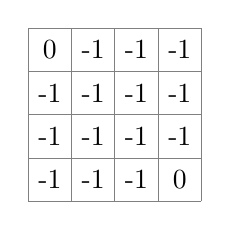
\begin{tikzpicture}[scale=1.1]
			\draw[step=0.5cm,color=gray] (-1,-1) grid (1,1);
			\node at (-0.75,+0.75) { 0 };
			\node at (-0.25,+0.75) {-1};
			\node at (+0.25,+0.75) {-1};
			\node at (+0.75,+0.75) {-1};
			\node at (-0.75,+0.25) {-1};
			\node at (-0.25,+0.25) {-1};
			\node at (+0.25,+0.25) {-1};
			\node at (+0.75,+0.25) {-1};
			\node at (-0.75,-0.25) {-1};
			\node at (-0.25,-0.25) {-1};
			\node at (+0.25,-0.25) {-1};
			\node at (+0.75,-0.25) {-1};

			\node at (-0.75,-0.75) {-1};
			\node at (-0.25,-0.75) {-1};
			\node at (+0.25,-0.75) {-1};
			\node at (+0.75,-0.75) { 0  };
			\end{tikzpicture}
		\end{column}
		\begin{column}{0.3\textwidth} 
			\begin{tikzpicture}[scale=1.1]
			\draw[step=0.5cm,color=gray] (-1,-1) grid (1,1);
			\node at (-0.75,+0.75) { \faFlagCheckered };
			\node at (-0.25,+0.75) { $\leftarrow$ };
			\node at (+0.25,+0.75) {?};
			\node at (+0.75,+0.75) {?};
			\node at (-0.75,+0.25) {$\uparrow$};
			\node at (-0.25,+0.25) {?};
			\node at (+0.25,+0.25) {?};
			\node at (+0.75,+0.25) {?};
			\node at (-0.75,-0.25) {?};
			\node at (-0.25,-0.25) {?};
			\node at (+0.25,-0.25) {?};
			\node at (+0.75,-0.25) {$\downarrow$};

			\node at (-0.75,-0.75) {?};
			\node at (-0.25,-0.75) {?};
			\node at (+0.25,-0.75) {$\rightarrow$};
			\node at (+0.75,-0.75) { \faFlagCheckered  };
			\end{tikzpicture}
		\end{column}
		\begin{column}{0.1\textwidth}
		\end{column}
	\end{columns}
	\vfill
	\begin{columns}
		\begin{column}{0.1\textwidth}
		\end{column}
		\begin{column}{0.2\textwidth}
			k = 2
		\end{column}
		\begin{column}{0.3\textwidth}
			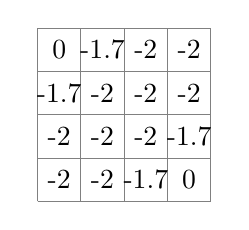
\begin{tikzpicture}[scale=1.1]
			\draw[step=0.5cm,color=gray] (-1,-1) grid (1,1);
			\node at (-0.75,+0.75) { 0 };
			\node at (-0.25,+0.75) {-1.7};
			\node at (+0.25,+0.75) {-2};
			\node at (+0.75,+0.75) {-2};
			\node at (-0.75,+0.25) {-1.7};
			\node at (-0.25,+0.25) {-2};
			\node at (+0.25,+0.25) {-2};
			\node at (+0.75,+0.25) {-2};
			\node at (-0.75,-0.25) {-2};
			\node at (-0.25,-0.25) {-2};
			\node at (+0.25,-0.25) {-2};
			\node at (+0.75,-0.25) {-1.7};

			\node at (-0.75,-0.75) {-2};
			\node at (-0.25,-0.75) {-2};
			\node at (+0.25,-0.75) {-1.7};
			\node at (+0.75,-0.75) { 0  };
			\end{tikzpicture}
		\end{column}
		\begin{column}{0.3\textwidth} 
			\begin{tikzpicture}[scale=1.1]
			\draw[step=0.5cm,color=gray] (-1,-1) grid (1,1);
			\node at (-0.75,+0.75) { \faFlagCheckered };
			\node at (-0.25,+0.75) { $\leftarrow$ };
			\node at (+0.25,+0.75) { $\leftarrow$ };
			\node at (+0.75,+0.75) {?};
			\node at (-0.75,+0.25) {$\uparrow$};
			\node at (-0.25,+0.25) {\includegraphics[scale=0.25]{img/left-up.png}	};
			\node at (+0.25,+0.25) {?};
			\node at (+0.75,+0.25) {$\downarrow$};
			\node at (-0.75,-0.25) { $\uparrow$ };
			\node at (-0.25,-0.25) {?};
			\node at (+0.25,-0.25) {\includegraphics[scale=0.25]{img/down-right.png}};
			\node at (+0.75,-0.25) {$\downarrow$};

			\node at (-0.75,-0.75) {?};
			\node at (-0.25,-0.75) {$\rightarrow$};
			\node at (+0.25,-0.75) {$\rightarrow$};
			\node at (+0.75,-0.75) { \faFlagCheckered  };
			\end{tikzpicture}
		\end{column}
		\begin{column}{0.1\textwidth}
		\end{column}
	\end{columns}
	\vfill
	\begin{columns}
		\begin{column}{0.1\textwidth}
		\end{column}
		\begin{column}{0.2\textwidth}
			k = 3
		\end{column}
		\begin{column}{0.3\textwidth}
			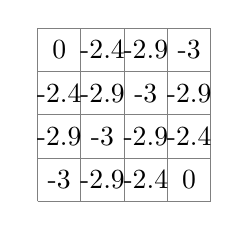
\begin{tikzpicture}[scale=1.1]
			\draw[step=0.5cm,color=gray] (-1,-1) grid (1,1);
			\node at (-0.75,+0.75) { 0 };
			\node at (-0.25,+0.75) {-2.4};
			\node at (+0.25,+0.75) {-2.9};
			\node at (+0.75,+0.75) {-3};
			\node at (-0.75,+0.25) {-2.4};
			\node at (-0.25,+0.25) {-2.9};
			\node at (+0.25,+0.25) {-3};
			\node at (+0.75,+0.25) {-2.9};
			\node at (-0.75,-0.25) {-2.9};
			\node at (-0.25,-0.25) {-3};
			\node at (+0.25,-0.25) {-2.9};
			\node at (+0.75,-0.25) {-2.4};

			\node at (-0.75,-0.75) {-3};
			\node at (-0.25,-0.75) {-2.9};
			\node at (+0.25,-0.75) {-2.4};
			\node at (+0.75,-0.75) { 0  };
			\end{tikzpicture}
		\end{column}
		\begin{column}{0.3\textwidth} 
			\begin{tikzpicture}[scale=1.1]
			\draw[step=0.5cm,color=gray] (-1,-1) grid (1,1);
			\node at (-0.75,+0.75) { \faFlagCheckered };
			\node at (-0.25,+0.75) { $\leftarrow$ };
			\node at (+0.25,+0.75) { $\leftarrow$ };
			\node at (+0.75,+0.75) {\includegraphics[scale=0.25]{img/down-left.png}};
			\node at (-0.75,+0.25) {$\uparrow$};
			\node at (-0.25,+0.25) {\includegraphics[scale=0.25]{img/left-up.png}	};
			\node at (+0.25,+0.25) {\includegraphics[scale=0.25]{img/down-left.png}};
			\node at (+0.75,+0.25) {$\downarrow$};
			\node at (-0.75,-0.25) { $\uparrow$ };
			\node at (-0.25,-0.25) {\includegraphics[scale=0.25]{img/down-right.png}};
			\node at (+0.25,-0.25) {\includegraphics[scale=0.25]{img/down-right.png}};
			\node at (+0.75,-0.25) {$\downarrow$};

			\node at (-0.75,-0.75) {\includegraphics[scale=0.25]{img/up-right.png}};
			\node at (-0.25,-0.75) {$\rightarrow$};
			\node at (+0.25,-0.75) {$\rightarrow$};
			\node at (+0.75,-0.75) { \faFlagCheckered  };
			\end{tikzpicture}
		\end{column}
		\begin{column}{0.1\textwidth}
		\end{column}
	\end{columns}
\end{frame}

\section{Neural Networks in RL}
\begin{frame}{Beyond the Gridworld}
	In the Gridworld every state value $\mathbf{v_t}$ is stored in a table. 
	The approach lacks scalability and is inherently limited to fairly low-dimension problems.
	\begin{figure}
		\includegraphics[scale=0.4]{img/dota2.jpg}
		\caption{The state $\mathbf{v_t}$ might be a frame of a videogame \cite{dota2}}
	\end{figure}
\end{frame}
\begin{frame}[fragile]{Deep Reinforcement Learning}
Deep  learning  enables  RL  to  scale  to  decision-making
problems  that  were  previously  intractable,  i.e.,  settings  with
high-dimensional  state  and  action  spaces. \cite{arulkumaran2017brief}
	\begin{itemize}
		\item Universal function approximator
		\item Representation learning
	\end{itemize}
	Neural networks can learn the approximated value of $\mathbf{V_s}$ or $\mathbf{Q(s, a)}$ for any given \textsc{state/action space}.
\end{frame}
\section{Actor-Critic}

\section{Deep Q-Learning}
\begin{frame}

\end{frame}
\begin{frame}[allowframebreaks]{References}

  \bibliography{rl}
  \bibliographystyle{abbrv}

\end{frame}

\begin{frame}[allowframebreaks]{List of Figures}
    \listoffigures
\end{frame}

\end{document}
